% Created by tikzDevice version 0.12.3 on 2020-06-04 22:56:01
% !TEX encoding = UTF-8 Unicode
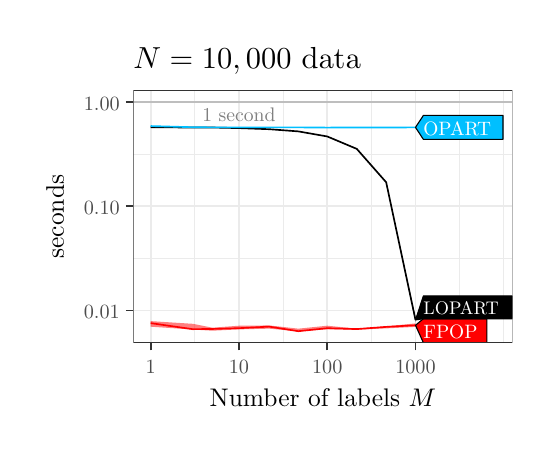
\begin{tikzpicture}[x=1pt,y=1pt]
\definecolor{fillColor}{RGB}{255,255,255}
\path[use as bounding box,fill=fillColor,fill opacity=0.00] (0,0) rectangle (180.67,144.54);
\begin{scope}
\path[clip] (  0.00,  0.00) rectangle (180.67,144.54);
\definecolor{drawColor}{RGB}{255,255,255}
\definecolor{fillColor}{RGB}{255,255,255}

\path[draw=drawColor,line width= 0.6pt,line join=round,line cap=round,fill=fillColor] (  0.00,  0.00) rectangle (180.68,144.54);
\end{scope}
\begin{scope}
\path[clip] ( 38.23, 30.69) rectangle (175.17,121.88);
\definecolor{fillColor}{RGB}{255,255,255}

\path[fill=fillColor] ( 38.23, 30.69) rectangle (175.18,121.88);
\definecolor{drawColor}{gray}{0.92}

\path[draw=drawColor,line width= 0.3pt,line join=round] ( 38.23, 61.19) --
	(175.17, 61.19);

\path[draw=drawColor,line width= 0.3pt,line join=round] ( 38.23, 98.89) --
	(175.17, 98.89);

\path[draw=drawColor,line width= 0.3pt,line join=round] ( 60.40, 30.69) --
	( 60.40,121.88);

\path[draw=drawColor,line width= 0.3pt,line join=round] ( 92.30, 30.69) --
	( 92.30,121.88);

\path[draw=drawColor,line width= 0.3pt,line join=round] (124.20, 30.69) --
	(124.20,121.88);

\path[draw=drawColor,line width= 0.3pt,line join=round] (156.09, 30.69) --
	(156.09,121.88);

\path[draw=drawColor,line width= 0.3pt,line join=round] (172.04, 30.69) --
	(172.04,121.88);

\path[draw=drawColor,line width= 0.6pt,line join=round] ( 38.23, 42.35) --
	(175.17, 42.35);

\path[draw=drawColor,line width= 0.6pt,line join=round] ( 38.23, 80.04) --
	(175.17, 80.04);

\path[draw=drawColor,line width= 0.6pt,line join=round] ( 38.23,117.74) --
	(175.17,117.74);

\path[draw=drawColor,line width= 0.6pt,line join=round] ( 44.45, 30.69) --
	( 44.45,121.88);

\path[draw=drawColor,line width= 0.6pt,line join=round] ( 76.35, 30.69) --
	( 76.35,121.88);

\path[draw=drawColor,line width= 0.6pt,line join=round] (108.25, 30.69) --
	(108.25,121.88);

\path[draw=drawColor,line width= 0.6pt,line join=round] (140.14, 30.69) --
	(140.14,121.88);
\definecolor{drawColor}{RGB}{190,190,190}

\path[draw=drawColor,line width= 0.6pt,line join=round] ( 38.23,117.74) -- (175.17,117.74);
\definecolor{drawColor}{gray}{0.50}

\node[text=drawColor,anchor=base,inner sep=0pt, outer sep=0pt, scale=  0.71] at ( 76.35,110.68) {1 second};
\definecolor{fillColor}{RGB}{255,0,0}

\path[fill=fillColor,fill opacity=0.50] ( 44.45, 38.50) --
	( 59.67, 37.53) --
	( 66.75, 36.12) --
	( 76.35, 36.84) --
	( 87.27, 36.94) --
	( 97.79, 35.78) --
	(108.25, 36.84) --
	(118.92, 35.79) --
	(129.54, 36.62) --
	(140.14, 37.67) --
	(140.14, 36.42) --
	(129.54, 35.88) --
	(118.92, 35.39) --
	(108.25, 35.58) --
	( 97.79, 34.83) --
	( 87.27, 35.78) --
	( 76.35, 35.52) --
	( 66.75, 35.04) --
	( 59.67, 35.46) --
	( 44.45, 36.49) --
	cycle;

\path[] ( 44.45, 38.50) --
	( 59.67, 37.53) --
	( 66.75, 36.12) --
	( 76.35, 36.84) --
	( 87.27, 36.94) --
	( 97.79, 35.78) --
	(108.25, 36.84) --
	(118.92, 35.79) --
	(129.54, 36.62) --
	(140.14, 37.67);

\path[] (140.14, 36.42) --
	(129.54, 35.88) --
	(118.92, 35.39) --
	(108.25, 35.58) --
	( 97.79, 34.83) --
	( 87.27, 35.78) --
	( 76.35, 35.52) --
	( 66.75, 35.04) --
	( 59.67, 35.46) --
	( 44.45, 36.49);
\definecolor{fillColor}{RGB}{0,0,0}

\path[fill=fillColor,fill opacity=0.50] ( 44.45,108.68) --
	( 59.67,108.51) --
	( 66.75,108.55) --
	( 76.35,108.25) --
	( 87.27,107.86) --
	( 97.79,107.07) --
	(108.25,105.27) --
	(118.92,100.83) --
	(129.54, 88.78) --
	(140.14, 40.05) --
	(140.14, 38.02) --
	(129.54, 88.68) --
	(118.92,100.66) --
	(108.25,105.21) --
	( 97.79,106.97) --
	( 87.27,107.80) --
	( 76.35,108.20) --
	( 66.75,108.41) --
	( 59.67,108.39) --
	( 44.45,108.51) --
	cycle;

\path[] ( 44.45,108.68) --
	( 59.67,108.51) --
	( 66.75,108.55) --
	( 76.35,108.25) --
	( 87.27,107.86) --
	( 97.79,107.07) --
	(108.25,105.27) --
	(118.92,100.83) --
	(129.54, 88.78) --
	(140.14, 40.05);

\path[] (140.14, 38.02) --
	(129.54, 88.68) --
	(118.92,100.66) --
	(108.25,105.21) --
	( 97.79,106.97) --
	( 87.27,107.80) --
	( 76.35,108.20) --
	( 66.75,108.41) --
	( 59.67,108.39) --
	( 44.45,108.51);
\definecolor{fillColor}{RGB}{0,191,255}

\path[fill=fillColor,fill opacity=0.50] ( 44.45,109.02) --
	( 59.67,108.67) --
	( 66.75,108.74) --
	( 76.35,108.55) --
	( 87.27,108.53) --
	( 97.79,108.55) --
	(108.25,108.51) --
	(118.92,108.49) --
	(129.54,108.48) --
	(140.14,108.51) --
	(140.14,108.47) --
	(129.54,108.43) --
	(118.92,108.47) --
	(108.25,108.43) --
	( 97.79,108.44) --
	( 87.27,108.45) --
	( 76.35,108.50) --
	( 66.75,108.48) --
	( 59.67,108.47) --
	( 44.45,108.83) --
	cycle;

\path[] ( 44.45,109.02) --
	( 59.67,108.67) --
	( 66.75,108.74) --
	( 76.35,108.55) --
	( 87.27,108.53) --
	( 97.79,108.55) --
	(108.25,108.51) --
	(118.92,108.49) --
	(129.54,108.48) --
	(140.14,108.51);

\path[] (140.14,108.47) --
	(129.54,108.43) --
	(118.92,108.47) --
	(108.25,108.43) --
	( 97.79,108.44) --
	( 87.27,108.45) --
	( 76.35,108.50) --
	( 66.75,108.48) --
	( 59.67,108.47) --
	( 44.45,108.83);
\definecolor{drawColor}{RGB}{255,0,0}

\path[draw=drawColor,line width= 0.6pt,line join=round] ( 44.45, 37.77) --
	( 59.67, 35.59) --
	( 66.75, 35.67) --
	( 76.35, 35.95) --
	( 87.27, 36.51) --
	( 97.79, 34.86) --
	(108.25, 35.94) --
	(118.92, 35.63) --
	(129.54, 36.42) --
	(140.14, 37.01);
\definecolor{drawColor}{RGB}{0,0,0}

\path[draw=drawColor,line width= 0.6pt,line join=round] ( 44.45,108.54) --
	( 59.67,108.47) --
	( 66.75,108.46) --
	( 76.35,108.25) --
	( 87.27,107.85) --
	( 97.79,107.06) --
	(108.25,105.23) --
	(118.92,100.74) --
	(129.54, 88.68) --
	(140.14, 38.93);
\definecolor{drawColor}{RGB}{0,191,255}

\path[draw=drawColor,line width= 0.6pt,line join=round] ( 44.45,108.99) --
	( 59.67,108.57) --
	( 66.75,108.51) --
	( 76.35,108.51) --
	( 87.27,108.50) --
	( 97.79,108.51) --
	(108.25,108.43) --
	(118.92,108.49) --
	(129.54,108.46) --
	(140.14,108.51);
\end{scope}
\begin{scope}
\path[clip] ( 38.23, 30.69) rectangle (175.17,121.88);
\definecolor{drawColor}{RGB}{0,0,0}
\definecolor{fillColor}{RGB}{255,0,0}

\path[draw=drawColor,line width= 0.4pt,line join=round,line cap=round,fill=fillColor] (140.14, 37.01) --
	(142.99, 39.36) --
	(165.94, 39.36) --
	(165.94, 30.69) --
	(142.99, 30.69) --
	cycle;
\definecolor{fillColor}{RGB}{0,0,0}

\path[draw=drawColor,line width= 0.4pt,line join=round,line cap=round,fill=fillColor] (140.14, 38.93) --
	(142.99, 47.60) --
	(175.18, 47.60) --
	(175.18, 39.36) --
	(142.99, 39.36) --
	cycle;
\definecolor{fillColor}{RGB}{0,191,255}

\path[draw=drawColor,line width= 0.4pt,line join=round,line cap=round,fill=fillColor] (140.14,108.51) --
	(142.99,112.84) --
	(171.76,112.84) --
	(171.76,104.17) --
	(142.99,104.17) --
	cycle;
\definecolor{drawColor}{RGB}{255,255,255}

\node[text=drawColor,anchor=base west,inner sep=0pt, outer sep=0pt, scale=  0.70] at (142.99, 32.13) {FPOP};

\node[text=drawColor,anchor=base west,inner sep=0pt, outer sep=0pt, scale=  0.66] at (142.99, 40.74) {LOPART};

\node[text=drawColor,anchor=base west,inner sep=0pt, outer sep=0pt, scale=  0.70] at (142.99,105.61) {OPART};
\definecolor{drawColor}{gray}{0.20}

\path[draw=drawColor,line width= 0.6pt,line join=round,line cap=round] ( 38.23, 30.69) rectangle (175.18,121.88);
\end{scope}
\begin{scope}
\path[clip] (  0.00,  0.00) rectangle (180.67,144.54);
\definecolor{drawColor}{gray}{0.30}

\node[text=drawColor,anchor=base east,inner sep=0pt, outer sep=0pt, scale=  0.73] at ( 33.28, 39.32) {0.01};

\node[text=drawColor,anchor=base east,inner sep=0pt, outer sep=0pt, scale=  0.73] at ( 33.28, 77.01) {0.10};

\node[text=drawColor,anchor=base east,inner sep=0pt, outer sep=0pt, scale=  0.73] at ( 33.28,114.71) {1.00};
\end{scope}
\begin{scope}
\path[clip] (  0.00,  0.00) rectangle (180.67,144.54);
\definecolor{drawColor}{gray}{0.20}

\path[draw=drawColor,line width= 0.6pt,line join=round] ( 35.48, 42.35) --
	( 38.23, 42.35);

\path[draw=drawColor,line width= 0.6pt,line join=round] ( 35.48, 80.04) --
	( 38.23, 80.04);

\path[draw=drawColor,line width= 0.6pt,line join=round] ( 35.48,117.74) --
	( 38.23,117.74);
\end{scope}
\begin{scope}
\path[clip] (  0.00,  0.00) rectangle (180.67,144.54);
\definecolor{drawColor}{gray}{0.20}

\path[draw=drawColor,line width= 0.6pt,line join=round] ( 44.45, 27.94) --
	( 44.45, 30.69);

\path[draw=drawColor,line width= 0.6pt,line join=round] ( 76.35, 27.94) --
	( 76.35, 30.69);

\path[draw=drawColor,line width= 0.6pt,line join=round] (108.25, 27.94) --
	(108.25, 30.69);

\path[draw=drawColor,line width= 0.6pt,line join=round] (140.14, 27.94) --
	(140.14, 30.69);
\end{scope}
\begin{scope}
\path[clip] (  0.00,  0.00) rectangle (180.67,144.54);
\definecolor{drawColor}{gray}{0.30}

\node[text=drawColor,anchor=base,inner sep=0pt, outer sep=0pt, scale=  0.73] at ( 44.45, 19.68) {1};

\node[text=drawColor,anchor=base,inner sep=0pt, outer sep=0pt, scale=  0.73] at ( 76.35, 19.68) {10};

\node[text=drawColor,anchor=base,inner sep=0pt, outer sep=0pt, scale=  0.73] at (108.25, 19.68) {100};

\node[text=drawColor,anchor=base,inner sep=0pt, outer sep=0pt, scale=  0.73] at (140.14, 19.68) {1000};
\end{scope}
\begin{scope}
\path[clip] (  0.00,  0.00) rectangle (180.67,144.54);
\definecolor{drawColor}{RGB}{0,0,0}

\node[text=drawColor,anchor=base,inner sep=0pt, outer sep=0pt, scale=  0.92] at (106.70,  7.64) {Number of labels $M$};
\end{scope}
\begin{scope}
\path[clip] (  0.00,  0.00) rectangle (180.67,144.54);
\definecolor{drawColor}{RGB}{0,0,0}

\node[text=drawColor,rotate= 90.00,anchor=base,inner sep=0pt, outer sep=0pt, scale=  0.92] at ( 13.08, 76.28) {seconds};
\end{scope}
\begin{scope}
\path[clip] (  0.00,  0.00) rectangle (180.67,144.54);
\definecolor{drawColor}{RGB}{0,0,0}

\node[text=drawColor,anchor=base west,inner sep=0pt, outer sep=0pt, scale=  1.10] at ( 38.23,129.95) {$N=10,000$ data};
\end{scope}
\end{tikzpicture}
